\documentclass{article}
\usepackage[utf8]{inputenc}
\textheight = 25cm 
\textwidth = 18cm
\topmargin = -3.0cm 
\oddsidemargin = 0.5cm
\usepackage{hyperref}
\hypersetup{
    colorlinks=true,
    linkcolor=blue,
    filecolor=blue,
    citecolor=black,      
    urlcolor=blue,
    }

\usepackage{float}
\usepackage{graphicx}

\usepackage{amsmath}
\usepackage{amssymb}
\usepackage{amsfonts}
\usepackage{mathtools, xparse}
\usepackage[shortlabels]{enumitem}

\usepackage[many]{tcolorbox}
\usepackage{lipsum}

\title{Tarea 4 Matemáticas Avanzadas de la Física}
\author{Cerritos Lira Carlos}
\date{7 de Abril del 2020}

\begin{document}
\maketitle
\subsection*{1.-}
Usando el método de Frobenius, encontrar la solución general en todos los casos de los 
parámetros de la denominada \textit{ecuación hipergeométrica}, dada por:
\[ x(1-x)y'' + [\gamma - (\alpha + \beta + 1)x]y' - \alpha \beta y = 0 \quad \alpha,\beta,\gamma \in C \]
Comprobar que las soluciones se escriben en términos de la \textit{función hipergeométrica de Gauss}, definida como:
\[ F(\alpha, \beta; \gamma; x) = \sum_{k=0}^\infty \frac{(\alpha)_k(\beta)_k}{(\gamma)_k} \frac{x^k}{k!}, \quad |x| < 1 \]
donde $(\lambda)_k$ denota el símbolo de \textit{Pochhammer}, definido recurrentemete por:
\[ (\lambda_0) = 1, \quad (\lambda)_k = \lambda(\lambda+1)...(\lambda+k-1), \quad k=1,2,... \]
\begin{tcolorbox}[breakable]
    Nuestra ecuación diferencial es de la forma:
    \[ y''(x) + p(x)y' + q(x)y = 0 \]
    donde:
    \[p(x) = \frac{\gamma - (\alpha + \beta + 1)x}{x(1-x)}\]
    \[q(x) = -\frac{\alpha \beta}{x(1-x)} \]
    obervamos que $f(x) = xp(x)$ y $g(x) = x^2q(x)$ son analíticas en $x=0$, por lo tanto es un punto singular regular,
    proponemos la solución:
    \begin{align*}
        y &= \sum_{n=0}^\infty a_nx^{n+s} \\
        y' &= \sum_{n=0}^\infty a_n(n+s)x^{n+s-1} \\
        y'' &= \sum_{n=0}^\infty a_n(n+s)(n+s-1)x^{n+s-2} 
    \end{align*}
    sustituyendo en la ecuación hipergeométrica obtenemos:
    \begin{align*}
        &\sum_{n=0}^\infty a_n(n+s)(n+s-1)x^{n+s-1} - \sum_{n=0}^\infty a_n(n+s)(n+s-1)x^{n+s} \\ 
        +\gamma &\sum_{n=0}^\infty a_n(n+s)x^{n+s-1} -(\alpha + \beta + 1)\sum_{n=0}^\infty a_n(n+s)x^{n+s} \\
        -\alpha \beta &\sum_{n=0}^\infty a_nx^{n+s} = 0
    \end{align*}
    movelos los índices para tener tener las mismas potenicas:
    \begin{align*}
        &\sum_{n=0}^\infty a_n(n+s)(n+s-1)x^{n+s-1} - \sum_{n=1}^\infty a_{n-1}(n+s-1)(n+s-2)x^{n+s-1} \\ 
        +\gamma &\sum_{n=0}^\infty a_n(n+s)x^{n+s-1} -(\alpha + \beta + 1)\sum_{n=1}^\infty a_{n-1}(n+s-1)x^{n+s-1} \\
        -\alpha \beta &\sum_{n=1}^\infty a_{n-1}x^{n+s-1} = 0    
    \end{align*}
    agrupando obtenemos:
    \begin{align*}
        a_0(s(s-1)+\gamma s) &= 0 \\
        ((n+s)(n+s-1)+\gamma(n+s))a_n + (-(n+s-1)(n+s-2)-(1+\alpha+\beta)(n+s-1)-\alpha \beta)a_{n-1} &= 0
    \end{align*}
    de la primer ecuación:
    \begin{align*}
        a_0(s(s-1)+\gamma c) &= 0 \\
        s(s-1) + \gamma) &= 0 \\
        s_1 = 0, \quad &s_2 = 1-\gamma
    \end{align*}
    agrupando términos obtenemos formula recurrente para $a_n$:
    \begin{align*}
        a_n &= \frac{(n+s-1)(n+s-2)+(1+\alpha+\beta)(n+s-1)}{(n+s)(n+s-1) + \gamma(n+s)}a_{n-1} \\
        a_n &= \frac{(n+s-1)(n+s+\alpha+\beta-1)+\alpha \beta}{(n+s)(n+s+\gamma-1)}a_{n-1} \\
        a_n &= \frac{(n+s+\alpha-1)(n+c+\beta - 1)}{(n+s)(n+s+\gamma-1)}a_{n-1} 
    \end{align*}
    en términos de $a_0$ obtenemos:
    \[ a_n = \frac{(s+\alpha)_n(s+\beta)_n}{(s+1)_n(s+\gamma)_n}a_0 \]
    finalmente la solución estaría dada por:
    \[ y = a_0 \sum_{n=0}^\infty \frac{(s+\alpha)_n(s+\beta)_n}{(s+1)_n(s+\gamma)_n} x^{n+s} \]
    de acuerdo al teorema de Fuchs tenemos que analizar $s_1-s_2$ para obtener las soluciones, en este 
    caso se reduce a analizar el comportamiento de $\gamma$.
    \subsubsection*{$\gamma \notin N_0$}
    Estamos en el caso $s_1 \neq s_2$ y $s_1-s_2 \notin N$. \\
    Para $s=0$ obtenemos:
    \begin{align*}
        y_1(x)
        &= a_0\sum_{n=0}^\infty \frac{(\alpha)_n (\beta)_n}{(\gamma)_n}x^{n} \\
        &= a_0F(\alpha, \beta; \gamma; x) 
    \end{align*}
    para $s=1-\gamma$
    \begin{align*}
        y_2(x)
        &= a_0x^{1-\gamma} \sum_{n=0}^\infty \frac{(\alpha+1-\gamma)_n(\beta + 1 - \gamma)_n}{(2-\gamma_n)}x^n \\
        &= a_0x^{1-\gamma}F(\alpha-\gamma+1, \beta-\gamma+1; 2-\gamma; x)
    \end{align*}
    \subsubsection*{$\gamma \in N_0$}
    \subsubsection*{$\gamma = 1$}
    Estamos en el caso $s_1=s_2$. \\
    Se tiene la solcuión:
    \begin{align*}
        y_1(x) 
        &= a_0 \sum_{n=0}^\infty \frac{(\alpha)_n (\beta)_n}{(1)_n} \\
        &= a_0 F(\alpha,\beta;1;x)
    \end{align*}
    Además se tiene una segunda solución:
    \begin{align*}
        y_2(x) = y_1(x)ln(x) + \sum_{n=0}^\infty a_n' x^{n}
    \end{align*}

\end{tcolorbox}

\subsection*{2.-}
Sea $y$ solución de la ecuación de Legendre $(1-x^2)y''-2xy'+ \nu(\nu+1)y=0, \nu \in R$
\begin{enumerate}[a)]
    \item Hacer el cambio de variable $t=\frac{1}{2}(1-x)$ en la ecuación diferencial de Legendre y 
    expresarla en términos de la ecuación hipergeométrica. Obtener una solución escrita en términos de la función 
    hipergeométrica de Gauss. A esta solución, que se denota por $P_\nu(x)$, se le denomina \textit{función de Legendre de grado $\nu$ de primera especie}.
    \item Hacer el cambio de variable $t=x^{-2}$ y $y=x^{-\nu-1}v$ en térmionos de la ecuación hipergeométrica. Obtener una solución escrita en términos de
    función hipergeométrica de Gauss. A esta solución, que se denota por $Q_\nu(x)$, se le denomina 
    \textit{función de Legendre de grado $\nu$ de segunda especie}.
    \item Hacer algunas gráficas representativas de las funciones $P_\nu(x)$ y $Q_\nu(x)$ para ciertos valores de $\nu$ a vuestra elección
    (no necesariamente enteros)
\end{enumerate}
\begin{tcolorbox}[breakable]
    \subsubsection*{a)}
        Veremos la ecuación que satisface $y(t)$, hacemos cuentas:
        \begin{align*}
            x(t) &= -2t+1 \\
            x'(t) &= -2 \\
            x''(t) &= 0
        \end{align*}
        donde $y(t) = y(x(t))$ $y(x) = y(t(x))$
        \begin{align*}
            y'(t) &= -2y'(x(t)) \\
            y''(t) &= 4y''(x(t))
        \end{align*}
        esta nueva función satisface la ecuación:
        \[ (1-(-2t+1)^2)\tfrac{1}{4}y'' + (-2t+1)y' + \nu(\nu+1)y = 0 \]
        desarrollando la expresión obtenemos:
        \begin{align*}
            \tfrac{1}{4}(1-(4t^2-4t+1))y'' + (1-2t)y' - (-\nu)(\nu+1)y &= 0 \\
            \tfrac{1}{4}(-4t^2+4t) + (1-2t)y' - (-\nu)(\nu+1)y &= 0 \\
            t(1-t)y'' + (1-2t)y' - (-\nu)(\nu+1)y &= 0 \\
        \end{align*}
        de donde el valor de los parámetros de la ecuación hipergeométrica:
        \[ \alpha = -\nu, \beta = \nu+1, \gamma = 1 \]
        se tiene por solución entonces:
        \begin{align*}
            y(x) 
            &= F(\alpha,\beta,\gamma, t(x)) \\
            &= F(-\nu, \nu+1, 1, \tfrac{1}{2}(1-x)), \quad |x|<1
        \end{align*}
    \subsubsection*{b)}
        Se tienen las siguientes relaciones:
        \begin{align*}
            y(x) &= x^{-\nu-1}v(x) \\
            y'(x) 
            &= (-\nu-1)x^{-\nu-2}v(x) + x^{-\nu-1}v'(x) \\
            &= (-\nu-1)x^{-1}y(x) + x^{-\nu-1}v'(x) \\
            y''(x) 
            &= (-\nu-1)(-\nu-2)x^{-\nu-3}v(x) + (-\nu-1)x^{-\nu-2}v'(x) + (-\nu-1)x^{-\nu-2}v'(x) + x^{-\nu-1}v''(x) \\
            &= (-\nu-1)(-\nu-2)x^{-2}y(x) + 2(-\nu-1)x^{-\nu-2}v'(x) + x^{-\nu-1}v''(x)
        \end{align*}
        como $y$ satisface la ecuación:
        \[ (1-x^2)y''-2xy'+ \nu(\nu+1)y=0 \]
        sustituyendo encontramos que $v$ satisface:
        \begin{align*}
            &\quad (1-x^2)((-\nu-1)(-\nu-2)x^{-2}y(x) + 2(-\nu-1)x^{-\nu-2}v'(x) + x^{-\nu-1}v''(x)) \\
            &+ (-2x)((-\nu-1)x^{-1}y(x) + x^{-\nu-1}v'(x)) \\
            &+ \nu(\nu+1)x^{-\nu-1}v(x) = 0 \\ \\ 
            &\quad (1-x^2)x^{-\nu-1}v''(x) \\
            &+(2(1-x^2)(-\nu-1)x^{-\nu-2}-2xx^{-\nu-1})v'(x) \\
            &+ ((1-x^2)((-\nu-1)(-\nu-2)x^{-2}v(x) + 2x(\nu+1)x^{-1} + \nu(\nu+1))x^{-\nu-1}v(x) = 0 \\ \\
            &\quad (1-x^2)v''(x) \\
            &+(2(1-x^2)(-\nu-1)x^{-1} - 2x)v'(x) \\
            &+ ((1-x^2)(\nu+1)(\nu+2)x^{-2} + 2(\nu+1) + \nu(\nu+1))v(x) = 0 
        \end{align*}
        haciendo el cambio de variable $t=x^{-2}$, veremos la ecuación que satisface $v(t)$, haciendo cuentas:
        \begin{align*}
            x(t) &= t^{-\frac{1}{2}} \\
            x'(t) &= -\frac{1}{2}t^{-\frac{3}{2}} \\ 
            x''(t) &= \frac{3}{2}t^{-\frac{5}{2}} \\
            v'(t) &= v'(x(t))x'(t) = -\frac{1}{2}v'(x(t))t^{-\frac{3}{2}} \\
            v''(t) &= v''(x(t))x'^2(t) + v'(x(t))x''(t) = \frac{1}{4} v''(x(t))t^{-3} + \frac{3}{2}v'(x(t))t^{-\frac{5}{2}}
        \end{align*}
        sustituyendo por $x(t)$ en la expresión que satisface $v$ obtenemos:
        \begin{align*}
            &\quad (1-t^{-1})v''(x(t)) \\
            &+((1-t^{-1})(-\nu-1)t^{\frac{1}{2}} - 2t^{-\frac{1}{2}})v'(x(t)) \\
            &+((1-t^{-1})(\nu+1)(\nu+2)t + 2(\nu+1) + \nu(\nu+1))v(x(t)) = 0 \\
            &\quad t(1-t)v''(t) 
            +\left(\nu + \frac{3}{2} -  \left[ \frac{\nu+1}{2}+\frac{\nu+2}{2}+1\right]t \right)v'(t) 
            -\frac{\nu+1}{2}\frac{\nu+2}{2}v(t) = 0
        \end{align*}
        $v$ sartisface la ecuación hipergeométrica con los parámetros:
        \[ \alpha = \frac{\nu+1}{2},\beta = \frac{\nu+2}{2}, \gamma = \nu+\frac{3}{2} \]
        finalmente obtenemos:
        \begin{align*}
            y(x) 
            &= x^{-\nu-1}v(x) \\
            &= \frac{1}{x^{\nu+1}}F\left(\alpha,\beta,\gamma, \frac{1}{x^2} \right) \\
            &= \frac{1}{x^{\nu+1}}F\left(\frac{\nu+1}{2}, \frac{\nu+2}{2}, \nu+\frac{3}{2}, \frac{1}{x^2} \right), \quad |x|>1
        \end{align*}
    \subsubsection*{c)}
    A continuación la gráfica de $P_\nu$
    \begin{figure}[H]
        \centering
        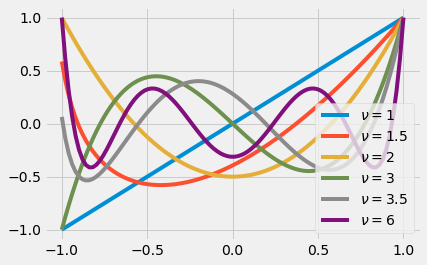
\includegraphics[scale=0.7]{images/p2_p.png}
        \caption{Gráfica $P_\nu$ para distintos valores de $\nu$}
    \end{figure}
\end{tcolorbox}

\subsection*{3.-}
\begin{enumerate}[a)]
    \item Demostrar la siguiente función generadora para las funciones de Bessel de primer especie con índice enetero:
    \[ e^{\frac{x}{2}(t-\frac{1}{t})} = \sum_{n=-\infty}^\infty J_n(x)t^n \]
    \item Usar la anterior función generadora y algunas herramientas de análsis complejo para derivar la siguiente representación integral 
    de las funciones de Bessel de primera especie:
    \[  J_n(x) = \frac{1}{\pi} \int_0^\pi cos(xsin\theta - n\theta)d\theta, \quad n \in Z \]
\end{enumerate}
\begin{tcolorbox}[breakable]
    \subsubsection*{a)}
    Realizaremos desarollo en serie de potencias para obtener una serie:
    \begin{align*}
        e^{\frac{1}{2}(t-\frac{1}{t})} 
        &= e^{\frac{xt}{2}}e^{-\frac{x}{2t}} \\
        &= \sum_{n=0}^\infty \frac{1}{n!}
        \left( \frac{xt}{2}\right)^n
        \sum_{n=0}^\infty \frac{1}{n!}
        (-1)^n \left(\frac{xt}{2}\right)^n \\
        &= \sum_{n=-\infty}^\infty a_n(x)t^n
    \end{align*}
    Encontramos $a_n$ usando el producto de Cauchy:
    \begin{align*}
        a_n(x) 
        &= \sum_{k=0}^\infty \frac{1}{(n+k)!} 
        \left( \frac{x}{2}\right)^{n+k}
        \frac{(-1)^k}{k!} \left( \frac{x}{2} \right)^k \\
        &= \sum_{k=0}^\infty \frac{(-1)^k}{\Gamma(k+1)\Gamma(k+n+1)} \left(\frac{x}{2}\right)^{2k+n} \\
        &= J_n(x)
    \end{align*}

    \subsubsection*{b)}
    Recordando el teorema del residuo, si una función tiene la representación:
    \[ f(z) = \sum_{n=-\infty}^\infty a_n(z-z_0)^n \]
    y $C$ una curva cerrada oriendata positiva que contiene a $z_0$, entonces:
    \[ \oint_C f(z)dz = 2\pi ia_{-1} \]
    Definimos y aplicamos el teorema a una función de tal forma que podamos despejar $J_n$:
    \begin{align*}
        \oint_C \frac{e^{\frac{x}{2}(t-\frac{1}{t})}}{t^{n+1}} dt 
        &= \oint_C \sum_{m=-\infty}^\infty J_m(x)t^{m-n-1} \\
        &= \oint_c \sum_{m=-\infty}^\infty J_{m+n+1}t^m \\
        &= 2\pi i J_n(x)
    \end{align*}
    elegimos a la curva $\gamma(\theta) = e^{i\theta}$, remplazando obtenemos:
    \begin{align*}
        \oint_C \frac{e^{\frac{x}{2}(t-\frac{1}{t})}}{t^{n+1}} dt 
        &= \int_0^{2\pi} \frac{e^{\frac{x}{2}(e^{i\theta}-e^{-i\theta})}}{e^{i\theta}e^{in\theta}} ie^{i\theta} d\theta \\
        &= i\int_{0}^{2\pi} e^{i(xsin\theta - n\theta)}d\theta 
    \end{align*}
    sustituyendo la expresión encontrada y despejando $J_n(x)$:
    \begin{align*}
        J_n(x)
        &= \frac{1}{2\pi} \int_0^{2\pi} e^{i(xsin\theta - n\theta)d\theta} \\
        &= \frac{1}{2\pi} \int_0^{2\pi} cos(xsin\theta - n\theta)d\theta + \frac{i}{2\pi}\int_0^{2\pi}sin(xsin\theta-n\theta)d\theta \\
        &= \frac{1}{\pi} \int_0^\pi cos(xsin\theta - n\theta)d\theta
    \end{align*}
\end{tcolorbox}

\subsection*{4.-}
Resolver la ecuación de Schrodinger estacionarie en coordenadas esféricas:
\[ -\frac{h^2}{2m} \nabla^2 \Psi (r,\theta,\phi) + V(r)\Psi(r,\theta,\phi) = E\Psi(r,\theta,\phi) \]
para el caso particular de potencial $V(r)=-\frac{e^2}{r}$ \textit{(átomo de hidrógeno)}, donde $e$ es la carga del electrón. 
Expresar las autofunciones en términos de ármonicos esféricos y polinimios ortogonales de Laguerre. Visualizar las órbitas de la función de onda del átomo de hidrógeno.
\begin{tcolorbox}[breakable]
    Usaremos coordenadas esféricas, además supondremos:
    \[ \Psi(r,\theta,\phi) = R(r)Y(\theta,\phi) \]
    La ecuación de Schrodinger se transforma en:
    \begin{align*}
    -\frac{\hbar^2}{2m}\left[
    \frac{Y}{r^2}\frac{d }{d r} \left( r^2\frac{\partial R}{\partial r} \right)    
    +\frac{R}{r^2sin\theta} \frac{\partial }{\partial \theta} \left( sin\theta \frac{\partial Y}{\partial \theta} \right)
    +\frac{R}{r^2sin^2\theta} \left(\frac{\partial^2 Y}{\partial \phi^2}\right)
    \right] + V\psi = E\psi 
    \end{align*}
    dividiendo entre $YR$ y multiplicando por $-\frac{2mr^2}{h^2}$ obtenemos:
    \begin{align*}
        \left[\frac{1}{R}\frac{d}{dr}\left( r^2\frac{dR}{dr} \right) - \frac{2mr^2}{\hbar^2}(V-E) \right]
        +\frac{1}{Y}\left[ \frac{1}{sin\theta}\frac{\partial }{\partial \theta} \left( sin\theta \frac{\partial Y}{\partial \theta} \right) + \frac{1}{sin^2\theta}\frac{\partial^2 Y}{\partial \phi^2}  \right]
        = 0
    \end{align*}
    en el lado izquierdo solo tenemos dependencia de $r$ y en el derecho solo de $\theta,\phi$, por lo tanto 
    deben ser constantes, llamaremos a esta constante $l(l+1)$. \\ 
    \subsubsection*{Ecuación ángular}
    La ecuación	para $Y$ es conocida y tiene por solución ármonicos esféricos:
    \[ Y_l^m(\theta, \phi) = \epsilon 
    \sqrt{\frac{2l+1}{4\pi} \frac{(l-|m|)!}{(l+|m|)!}}
    e^{im\phi}P_l^mcos(\theta) \]
    donde $\epsilon = (-1)^m, m\geq 0$ y $\epsilon = 1, m \leq 0$
    
    \subsubsection*{Ecuación radial}
    Recordando $R$ satisface la euación:
    \[ \frac{d}{dr}\left( r^2\frac{dR}{dr} \right) - \frac{2mr^2}{\hbar^2}(V-E)R = l(l+1)R \]
    realizando el cambio de variable:
    \[ u(r) = rR(r) \]
    la ecuación se transforma:
    \begin{align*}
        -\frac{\hbar^2}{2m} \frac{d^2u}{dr^2} + \left[ V + \frac{\hbar^2}{2m}\frac{l(l+1)}{r^2} - E \right]u &= 0 \\ 
        -\frac{\hbar^2}{2m} \frac{d^2u}{dr^2} + \left[ -\frac{e^2}{4\pi \epsilon_0}\frac{1}{r} + \frac{\hbar^2}{2m}\frac{l(l+1)}{r^2} - E \right]u &= 0 
    \end{align*}
    definimos:
    \[ k = \frac{\sqrt{-2mE}}{\hbar},\quad p = kr,\quad p_0 = \frac{me^2}{2\pi \epsilon_0\hbar^2k} \]
    realziando el cambio de variable y multiplicando por $\frac{2m}{\hbar^2}$ la ecuación se transforma:
    \[ \frac{d^2u}{dp^2} = \left[ 1- \frac{p_0}{p} + \frac{l(l+1)}{p^2} \right]u \]
    supondremos $u$ es de la forma:
    \[ u(p) = p^{l+1}e^{-p}v(p) \]
    realizando el cambio de variable la ecuación se transforma:
    \[ p\frac{d^2v}{dp^2} + 2(l+1-p)\frac{dv}{dp} + (p_0-2(l+1))v = 0 \]
    finalmente si $x=2p$ tenemos:
    \[ x\frac{d^2v}{dx^2} + (2(l+1)-x)\frac{dv}{dx} + \left( \frac{1}{2}p_0 - (l+1) \right)v = 0 \]
    ahora bien, el polinomio $L_n^k$ de Leguerre satisface:
    \begin{align*}
        x\frac{d^2}{dx^2}L_n^k(x) + (k+1-x)\frac{dL_n^k(x)}{dx} + nL_n^k(x) &= 0
    \end{align*}
    si hacemos:
    \[ k+1 = 2(l+1),\quad \bar{n} = \frac{1}{2}p_0 -(l+1) \]
    de la segunda condición debe ocurrir que $p_0 = 2n$, donde $n$ es un entero lo que implica:
    \[ E = -\frac{me^4}{32 \epsilon_0\hbar^2 \pi^2 n^2} \]
    \[ k = \frac{1}{an}, \quad a = \frac{4\pi \epsilon_0\hbar^2}{me^2} \]
    donde definimos:
    \[ E_n = -\left[ \frac{m}{2\hbar^2}\left( \frac{e^2}{4\pi \epsilon_0} \right)^2 \right] \frac{1}{n^2} = \frac{E_1}{n^2} \]
    entonces la solución esta dada por:
    \[ v(x) = L^{2l+1}_{n-(l+1)}(x) \]
    Finalmente escribimos la solución a la ecuación de Schrodinger:
    \[ \Psi_{nlm}(r, \theta, \phi) = \sqrt{\left( \frac{2}{na} \right)^3 \frac{(n-l-1)!}{2n[(n+1)!]}}e^{-\frac{r}{na}} \left(\frac{2r}{na}\right)^l L_{n-l-1}^{2l+1} \left( \frac{2r}{na} \right) Y_{l}^m(\theta,\phi) \]
    podemos visualizar el valor de $\Psi_{nlm}^2$ donde el brillo en cada región esta relacionado con la probabilidad de encontrar el electrón en dicha región. 
    \begin{figure}[H]
        \centering
        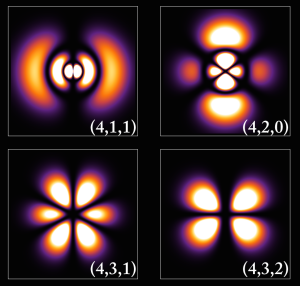
\includegraphics[scale=0.7]{images/p4_graph.png}
        \caption{Visualización densidad de probabilidad para disntintos valores de $nlm$}
    \end{figure}
\end{tcolorbox}

\end{document}
